\documentclass{article}

\usepackage[margin=1.0in]{geometry}
\usepackage{graphicx}
\usepackage{amsmath}
\usepackage{float}
\usepackage{enumitem}
\usepackage{gensymb}

\title{CSC 577 HW8}
\date{3/27/2019}
\author{Simon Swenson}

\begin{document}

\pagenumbering{gobble}
\maketitle
\pagenumbering{arabic}

\section{Introduction}

\begin{figure}[!ht]
	\centering
	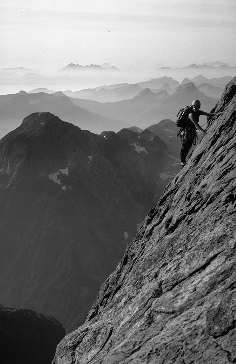
\includegraphics[width=60mm]{figs/climber_im.png}
	\caption{The climbing scene used in this assignment.}
\end{figure}

In this assignment, we explored convolutions, including how they could be used to detect 
edges, how they could reduce noise by applying Gaussian filters, and how they could 
be combined into a single filter. I completed all parts of the assignment. I 
chose the Lorem Ipsum text (C2) for the grad student portion.

If the text references an image that follows, but there is no image, please 
check the proceeding couple of pages. Latex is really annoying where it puts its 
images. I've tried to correct this in the past, but there's not a super 
straightforward way to do so without adding a bunch of newlines in the text which 
become stale if/when I modify the text and/or images.

Side note: I decided to use GNU Octave for this, which is a free implementation 
of MATLAB. If you find that the program doesn't work in MATLAB, please let me 
know. It could be as simple as removing the "pkg load statistics;" line.

\section{Part B}

\subsection{B.1}

Here, we compute the magnitude of the gradient of the image. Note that the 
gradient is a vector function. That is, it will output a vector for each pixel 
of the input image. We originally applied two convolutions, one that measures 
change in the x-direction and one that measures change in the y-direction. Since 
these are convolutions, we essentially want to make sure that when they're flipped, 
they're oriented how we want. Ideally, 
the x filter would be a vector of form [1.0 -1.0] and the y filter would be a vector 
of form [1.0; -1.0], but, to ensure that the response images were the same size to 
make computing the gradient easier, we made these filters both 2x2. The filters 
and their responses are shown below.

\begin{figure}[!ht]
	\centering
	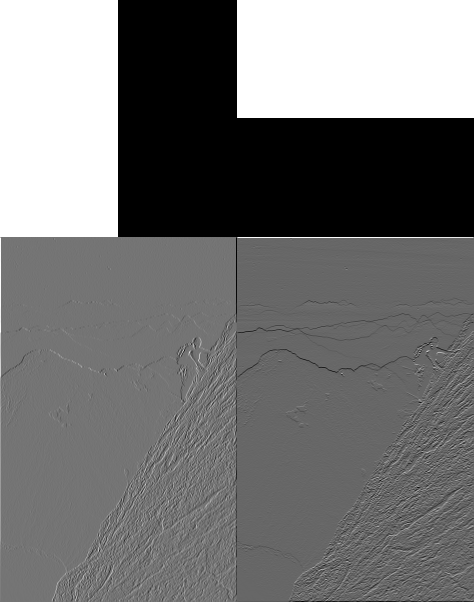
\includegraphics[width=100mm]{figs/dx_dy_filters_no_blur.png}
	\caption{The convolutions (top) and the responses when applied to the image 
        (bottom). Left estimates dx, right estimates dy.}
\end{figure}

After these were computed, the gradient magnitudes were computed using euclidean 
distance. The gradient magnitude image is shown below.

\begin{figure}[!ht]
	\centering
	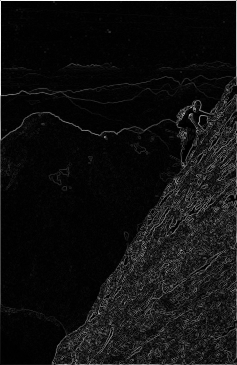
\includegraphics[width=60mm]{figs/gradient_magnitude.png}
	\caption{The magnitude of the gradient.}
\end{figure}

\subsection{B.2}

Now that we have gradient magnitudes, we can attempt to find edges, essentially 
those pixels in the image where the gradient magnitude is large (indicating a 
large change). This required a bit of trial and error to find a good threshold. 
Eventually, I settled on a threshold value of 0.35. This caught some of the 
smaller details of the image, including the high-frequency rock face.

\begin{figure}[!ht]
	\centering
	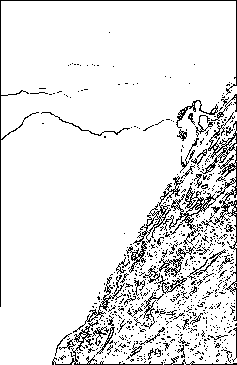
\includegraphics[width=60mm]{figs/threshold_response.png}
	\caption{A threshold of 0.35 applied to the gradient magnitude image. This 
        caught the background mountain outline, the outline of the climber, and 
        many of the high-frequency changes in the rock face.}
\end{figure}

\subsection{B.3}

For this section of the assigment, we experimented on blurring the input image 
to examine the image at a different scale. This required creating a function 
that would create a convolution representing a 2-d Gaussian distribution, given 
a sigma value. I made use of meshgrid and mvnpdf to make things easier. Below is 
the image after being blurred with a Gaussian filter with standard deviation 2.

\begin{figure}[!ht]
	\centering
	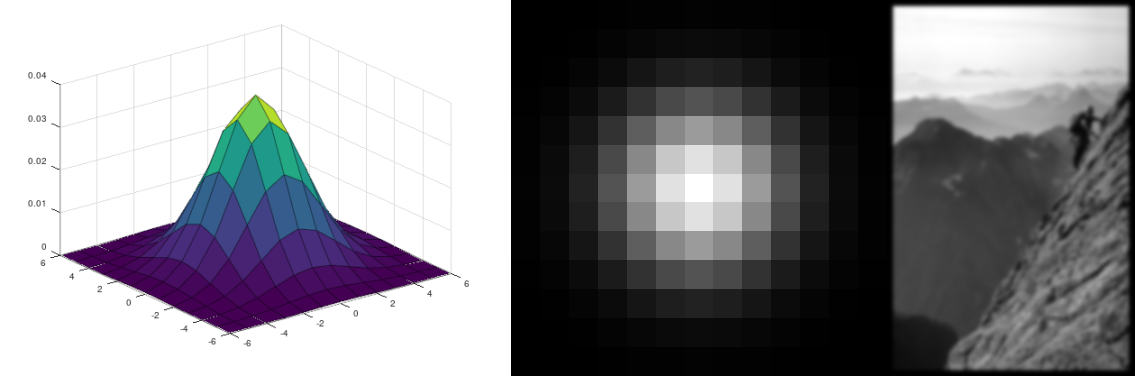
\includegraphics[width=160mm]{figs/gaussian_and_smoothed.png}
	\caption{A Gaussian with standard deviation 2. A plot of the 2-d Gaussian, represented in 3-d space (left), the corresponding kernel (center), and the 
        corresponding response image on the right, noticeably blurrier than the 
        initial image.}
\end{figure}

\subsection{B.4}

Here, we explored edge-finding with the blurred image above. The key is that this 
process found edges at a different image scale than the original edge detector. 
Essentially, this found edges at a higher scale, so the high-frequency edges of 
the cliff face are no longer as prevalent. Instead, the edges of the background 
mountain and the climber are more prominent in this image. In addition, we needed 
to use a lower threshold value to capture the edges at all. This is due to the 
Gaussian filter smoothing everything out, meaning the gradients will generally 
have a lower magnitude. The threshold value used here was 0.08.

\begin{figure}[!ht]
	\centering
	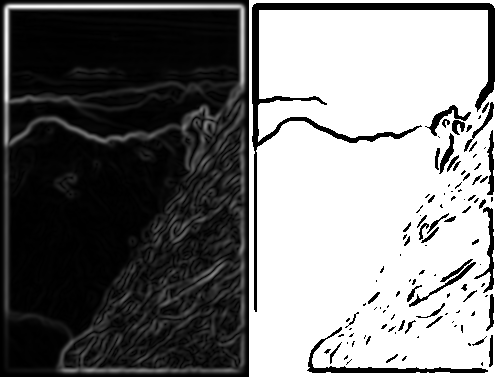
\includegraphics[width=100mm]{figs/smoothed_grad_mag_and_threshold.png}
	\caption{Left: The gradient magnitudes after applying the Gaussian filter 
        and the edge detector. Right: The edges found after setting a threshold of 0.08.}
\end{figure}

\subsection{B.5}

Here, instead of applying the Gaussian filter to the image, then the edge detector 
filters on that response, we use the associative property of convolutions to instead 
create a single filter, first convolving the Gaussian filter with the edge detector, 
then finally applying that combined filter to the image. In addition, we use a 
standard deviation of 4 instead of 2 for the Gaussian, making this filter even 
blurrier than the filter above. Here, I had to use an even lower threshold value 
due to the blurrier output image. I chose a value of 0.05. The two combined filters as well as the gradient 
magnitude image and edge threshold image are shown below.

\begin{figure}[!ht]
	\centering
	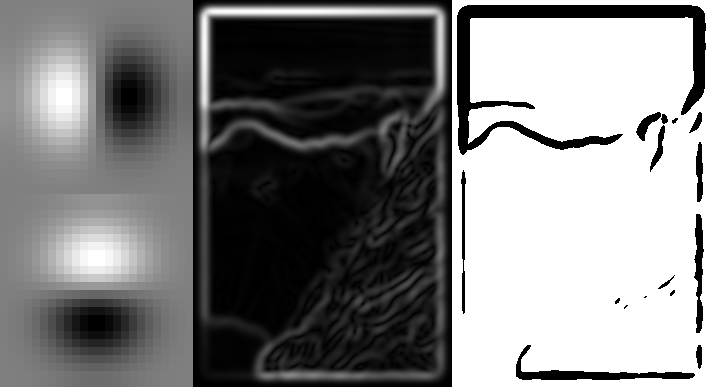
\includegraphics[width=120mm]{figs/smoothed_grad_mag_and_threshold_2.png}
	\caption{Left: The two combined filters created by convolving the Gaussian 
        filter with the horizontal edge detector (top-left) and the vertical edge 
        detector (bottom-left). Center: The gradient magnitudes after applying 
        the combined filters 
        (Gaussian with standard deviation 4 and edge detectors). Right: The edges 
        found after setting a threshold of 0.05.}
\end{figure}

\subsection{B.6}

It may be desireable to save some computation cost by applying 1-d convolutions 
instead of 2-d convolutions. It turns out this can easily be done with a 2-d 
Gaussian. In fact, the 2-d Gaussian is essentially two 1-d Gaussians multiplied 
together. Consider the PDF for the 2-d Gaussian filter that we used:

$$
f(\vec{x}) = (2 \pi)^{-\frac{k}{2}} det(\Sigma)^{-\frac{1}{2}} e^{-\frac{1}{2}(\vec{x} - \mu)^T \Sigma^{-1} (\vec{x} - \mu)}
$$

Now, we plug in some values for our particular case.

\begin{align*}
    k      &= 2 \\
    \Sigma &= \begin{bmatrix}
                  \sigma^2 &        0 \\
                         0 & \sigma^2
              \end{bmatrix} \\
    \mu    &= \vec{0}
\end{align*}

In addition, we can quickly calculate some values:

\begin{align*}
    det(\Sigma) &= \frac{1}{\sigma^4} \\
    \Sigma^{-1} &= \frac{1}{\sigma^4} \begin{bmatrix}
                                          \sigma^2 &        0 \\
                                                 0 & \sigma^2
                                      \end{bmatrix}
\end{align*}

This greatly simplifies the function $f(x)$ above:

\begin{align*}
f(\vec{x}) &= (2 \pi)^{-\frac{2}{2}} (\sigma^4)^{-\frac{1}{2}} e^{-\frac{1}{2} \vec{x}^T \frac{1}{\sigma^4} \begin{bmatrix}
            \sigma^2 &        0 \\
                   0 & \sigma^2
        \end{bmatrix} \vec{x}}
\end{align*}

Let's parameterize the function in terms of two variables, x, y, instead of a 
single vector variable:

\begin{align*}
f(x, y) &= (2 \pi)^{-\frac{2}{2}} (\sigma^4)^{-\frac{1}{2}} e^{-\frac{1}{2} \begin{bmatrix} x & y \end{bmatrix} \frac{1}{\sigma^4} \begin{bmatrix}
            \sigma^2 &        0 \\
                   0 & \sigma^2
        \end{bmatrix} \begin{bmatrix} x \\ y \end{bmatrix}} \\
        &= ((2 \pi)^{-\frac{1}{2}})^2 \sigma^{-2} e^{-\frac{1}{2 \sigma^4} (\sigma^2 x^2 + \sigma ^2 y^2)} \\
        &= ((2 \pi)^{-\frac{1}{2}})^2 (\sigma^{-1})^2 e^{-\frac{x^2}{2 \sigma^2}} e^{-\frac{y^2}{2 \sigma^2}} \\
        &= ((2 \pi)^{-\frac{1}{2}} \sigma^{-1} e^{-\frac{x^2}{2 \sigma^2}}) ((2 \pi)^{-\frac{1}{2}} \sigma^{-1} e^{-\frac{y^2}{2 \sigma^2}})
\end{align*}

Here, we have a clear separation of g(x) and h(y). In addition, these two are 
symmetric, so we really only need to calculate one equation (and then apply it in two different directions). In fact, it turns out that these 
are just two single-variate Gaussian distributions. From here, we can use MATLAB's 
builtin normpdf to get a 1-d convolution. We reshape this convolution to suit the 
dimension that we're considering, applying it once along the y-axis and once 
along the x-axis. The result is very good. This also saves us a lot of 
computation, since we're only using a 1-d convolution instead of a 2-d one.

\begin{figure}[!ht]
	\centering
	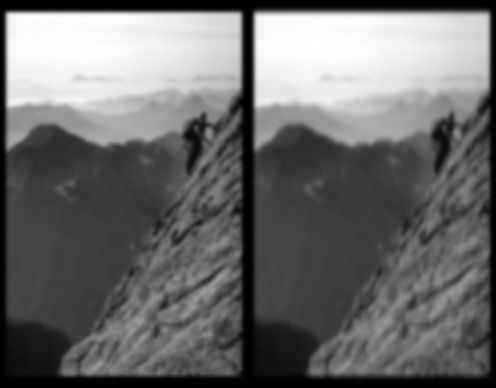
\includegraphics[width=100mm]{figs/2d_vs_2x_1d_blurs.png}
	\caption{Left: The original blur applied from earlier in the assignment. 
        Right: The blur applied as two 1-d convolutions. In theory, this should 
        be the same, but, to me, it looks slightly blurrier. This might just be 
        down to floating point errors. I'm not exactly sure.}
\end{figure}

\section{Part C2}

Here, we explored using correlation to create rudamentary OCR (optical character 
recognition). Since vowels are very common in words, I decided to pick a, e, i, 
o, and u for the five characters. I also wanted to use MATLAB's builtin conv2 
function, but that would cause a problem by naively using the raw images cropped 
out. First, the responses do not sum to 0. Second, since conv2 is a convolution, 
it flips the filter horizontally and vertically before applying it. This creates 
two pre-processing steps that we need to do: Subtract the mean from the five 
letter images and flip them horizontally and vertically. Additionally, we may 
want to scale the filter values to be in a reasonable range like [-1, 1].

After pre-processing the filters, we simply apply each one to the lorem ipsum 
image in turn. This doesn't give us exact letter matches, however. Instead, it 
gives us response values that range over an arbitrary range of values. From here, 
we must decide the best thresholds to use to ensure that each letter response 
captures all the corresponding letters and only those letters. At this point, I 
converted the text in the image to a .txt document manually so that I could count 
the occurrences of each letter to give me a better target. The totals are below:

\begin{tabular}{r | r}
    letter & count \\
    \hline         \\
         a &   155 \\
         e &   195 \\
         i &   205 \\
         o &    79 \\
         u &   166
\end{tabular}

To find a good threshold, I perform a binary search on the threshold range. I 
begin at the midpoint of the threshold range and count the number of pixels 
above that value. If the count is too high, I raise the threshold so that it's halfway 
between the old midpoint and the old max threshold. I also update the min to be the old midpoint. If the count is too low, I 
lower the threshold so that it's halfway between the old midpoint and the old 
min threshold. I also update the max to be the old midpoint.

All five letter responses converged at different thresholds:

\begin{tabular}{r | r}
    letter & threshold \\
    \hline             \\
         a &    7.5699 \\
         e &    6.8359 \\
         i &    1.9289 \\
         o &    9.4510 \\
         u &    7.0647
\end{tabular}

One thing that I found quite strange is the low threshold value for i. This 
could be caused by a number of things. First, i is a letter that doesn't have as 
many pixels as the other letters, so its response vector will naturally be lower, 
especially if we scale all pixels in the filter to be within [-1, 1] as I 
explained above. Second, anti-aliasing could cause quite a problem with 
such a small, vertical letter. Depending on where it appears on the line, it could 
cover two pixels horizontally, anti-aliased, or only one. This might affect the results.

After finding these thresholds, I created a color-coded response map over the 
original lorem ipsum text (below). This gave me a quick way of identifying where 
certain letter filters had problems.

\begin{figure}[!ht]
	\centering
	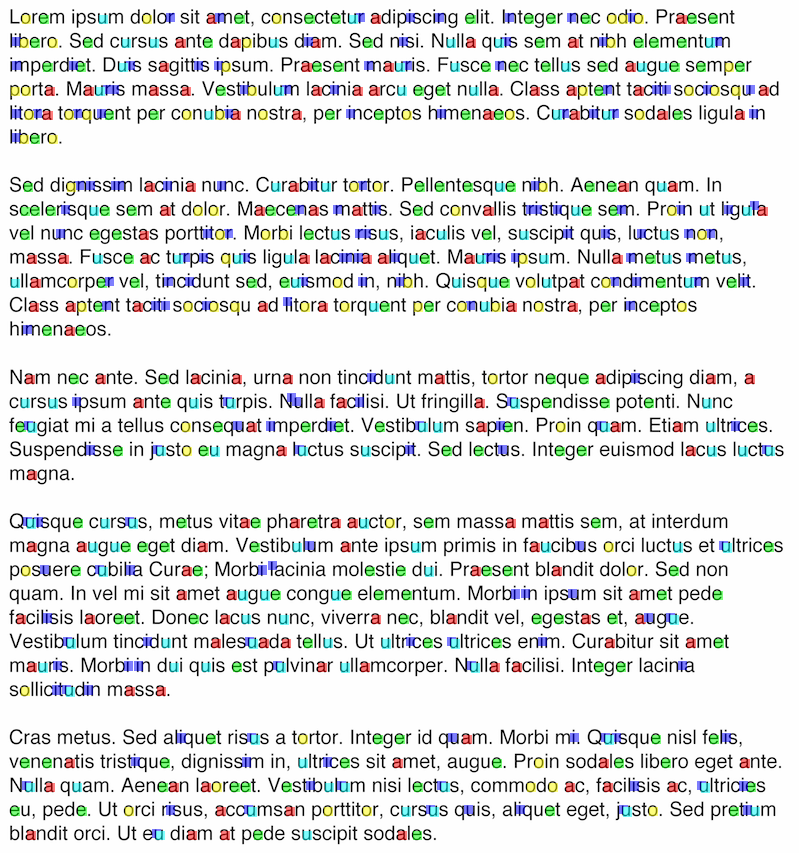
\includegraphics[width=160mm]{figs/lorem_ipsum_colors.png}
	\caption{The original lorem ipsum image with filter responses overlayed 
        transparently above. Red: a, green: e, blue: i, yellow: o, cyan: u.}
\end{figure}

From here, it was difficult to follow the spec of the assignment exactly. It 
stated that letters in the image which matched more than one filter should have 
the highest filter value selected, but, without the image being manually 
segmented into ranges of indices which represent each letter, it's hard to do 
this, since the filter responses do not line up exactly. If a letter had multiple 
responses to the filters, I just used the letter that happened to have its square 
overlayed last (in the order: red (a), green (e), blue (i), yellow (o), cyan (u)).

From here, we can painstakingly calculate the confusion matrix:

\begin{tabular}{r | r r r r r}
      &   a &   e &  i &  o &   u \\
    \hline                        \\
    a & 134 &   0 &  0 &  0 &   0 \\
    e &   0 & 161 &  0 &  0 &   0 \\
    i &   0 &   0 & 91 &  0 &  14 \\
    o &   0 &   0 &  0 & 55 &   0 \\
    u &   0 &   0 &  0 &  0 & 118
\end{tabular}

The confusion matrix looks roughly diagonal, but that's due to the fact that it 
only includes the five vowels. If we were to do a filter for every character, it 
would look much worse.

Some characters did better than others. However, comparing to the true numbers of 
each of the five letters (above), no filter was perfect. Letters with more 
intricate features like "a" and "e" performed better. However, the "i" filter had an 
especially hard time. Since many letters have vertical bars, "i" often caught those. 
In fact, "i" would often report positives for "u." "O" had similar problems, since 
many characters have some sort of circle feature. It would often catch p's, b's, 
and d's.

This filter approach is a good first step, but it does not handle anti-aliasing 
very well, which leads to many false positives and false negatives.

\end{document}